\documentclass{article}

% if you need to pass options to natbib, use, e.g.:
% \PassOptionsToPackage{numbers, compress}{natbib}
% before loading nips_2016
%
% to avoid loading the natbib package, add option nonatbib:
% \usepackage[nonatbib]{nips_2016}

\usepackage[final]{nips_2016}

% to compile a camera-ready version, add the [final] option, e.g.:
% \usepackage[final]{nips_2016}

\usepackage[utf8]{inputenc} % allow utf-8 input
\usepackage[T1]{fontenc}    % use 8-bit T1 fonts
\usepackage{hyperref}       % hyperlinks
\usepackage{url}            % simple URL typesetting
\usepackage{booktabs}       % professional-quality tables
\usepackage{amsfonts}       % blackboard math symbols
\usepackage{nicefrac}       % compact symbols for 1/2, etc.
\usepackage{microtype}      % microtypography
\usepackage{graphicx}


\title{Recursive Stacked Adversarial Network for Conditional Video Generation}

% The \author macro works with any number of authors. There are two
% commands used to separate the names and addresses of multiple
% authors: \And and \AND.
%
% Using \And between authors leaves it to LaTeX to determine where to
% break the lines. Using \AND forces a line break at that point. So,
% if LaTeX puts 3 of 4 authors names on the first line, and the last
% on the second line, try using \AND instead of \And before the third
% author name.

\author{
  Shujon Naha \\
  Department of Computer Science\\
  Indiana University\\
  Bloomington, IN \\
  \texttt{snaha@iu.edu} \\
  %% examples of more authors
   \And
   Khandokar Md. Nayem \\
  Department of Computer Science\\   
  Indiana University\\
  Bloomington, IN \\
   \texttt{knayem@iu.edu} \\
   \AND
   Md. Lisul Islam\\
  Department of Computer Science\\   
  Indiana University\\
  Bloomington, IN \\
   \texttt{islammdl@indiana.edu } \\
}

\begin{document}
% \nipsfinalcopy is no longer used

\maketitle

\begin{abstract}
  Generating video frames based on a pre-condition is a challenging problem and requires understanding of per frame contents and visual dynamics and their relevacies to the pre-condition. In this project, we propose a novel recurrent stacked adversarial network based model to generate video frames based on a given pre-condition. In our knowledge, this is the first work to address the problem of conditional video generation using adversarial network.
\end{abstract}


\section{Introduction}
Generative adversarial networks have been shown incredible results to produce images from pre-conditions such as text, attributes etc \cite{stackGAN, attribute2image}. In these works, random noises incorporated with a semantic vector representation of the prec-condition is given as input to the generator network to produce images relevant to the pre-condition. The discriminator network then learns to distinguish between the images generated by the generator and the real image from the database. A min-max learning algorithm is used to train these both models where the generator tries to continously fool the discriminator by producing better images similar to the original one and the discriminator learns to make the job harder for the generative network by getting better at distinguishing real and fake images. Most of the times, the generative network is a convolutional neural network which produces image from a single vector by using several deconvolution steps. The discriminator network is also a convolutional neural network which takes the image from the generator network output and the corresponding original image from the database and tells the similarity between the generated image and the real image. 


Generative adversarial networks have been also used for predicting future frames from a video sequence and generate videos with scene dynamics \cite{deepMSE, genVSD}. In this works, multiple frames are combined together and 3D convolution is used in the domains of space and time to predict the next frames. These works have shown the capability of adversarial networks to capture the scene dynamics although for small temporal intervals.

\begin{figure}[h]
  \centering
  %%\fbox{\rule[-.5cm]{0cm}{4cm} \rule[-.5cm]{4cm}{0cm}}
  \includegraphics[scale=0.5]{problem.png} 
  \caption{Generating video sequence based on a given pre-condition (sentence description).}
    \label{problem}
\end{figure}

In this project, we address the problem of generating videos based on pre-conditions such as action classes, fMRI signals and sentence descriptions using adversarial network. Generating videos based on pre-conditions pose a unique set of challenges than the conditional image generation and unconditional video generation problem. In our case, each of the frames will be generated based on the previous frames and the given pre-condition such as in Figure \ref{problem}. The numbers of previous frames can vary from zero to a maximum number. Thus the usual approach of using 3D convolution will not be applicable in our case. Moreover, we need to make the pre-condition available to the system at each time frame so the whole generated video is consistent with the pre-condition.    

%%\section{Related Works}
%%\label{related_works}


\section{Our Approach}
\label{our_approach}
In our problem, we are given a pre-condition either in the form of an action class name, fMRI signal or textual description and we need to generate a sequence of video frames which will be coherent with the given pre-condition. First, we will discuss how we can generate a high resolution frame independently based on the pre-condition using a stacked adversarial network. Then we will discuss how we can make a recurrent fully convolutional network so we can propagate the context to generate the next frame. Finally, we will describe our recurrent stacked adversarial network to generate videos based on pre-conditions.

\begin{figure}[h]
  \centering
  %%\fbox{\rule[-.5cm]{0cm}{4cm} \rule[-.5cm]{4cm}{0cm}}
  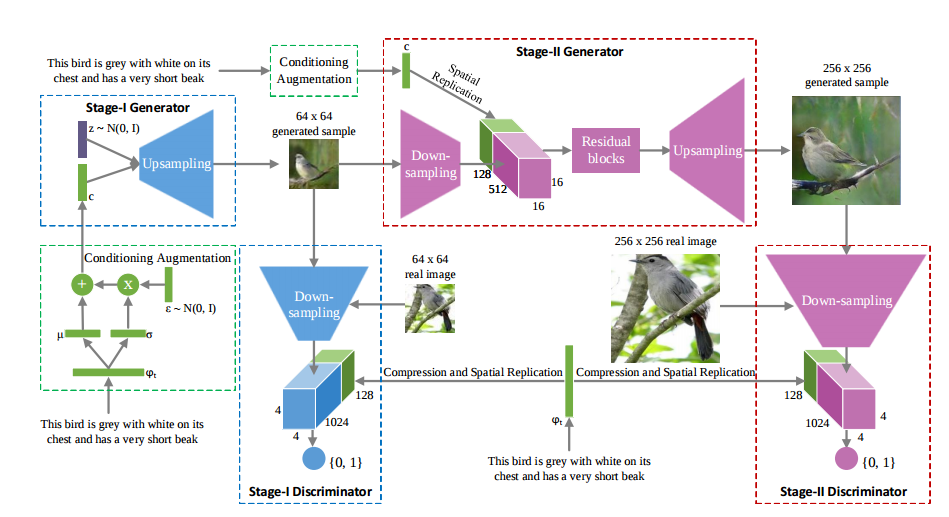
\includegraphics[scale=0.4]{stackgan.png} 
  \caption{The architecture of the StackGAN from \cite{stackGAN}. The Stage-I generator draws a low resolution image by sketching rough shape and basic colors of the object from the given text and painting the background from a random noise vector. The Stage-II generator generates a high resolution image with photo-realistic details by conditioning on both the Stage-I result and the text again.}
    \label{stackgan}
\end{figure}

\subsection{Stacked Adversarial Network}
To generate a video first, we need to learn to generate a single frame from the pre-condition. We have adapted the  StackGAN adversarial network model \cite{stackGAN} for this problem, as it can generate photo-realistic images from sentence descriptions. At first stage, this model generates an image based on the encoded text and a random vector. Then the generated image in the first stage is used as the input with the encoded text vector to the second stage adversarial network to generate a photo-realistic image. The architecture of the model can be seen in Figure \ref{stackgan}.

\begin{figure}[h]
  \centering
  %%\fbox{\rule[-.5cm]{0cm}{4cm} \rule[-.5cm]{4cm}{0cm}}
  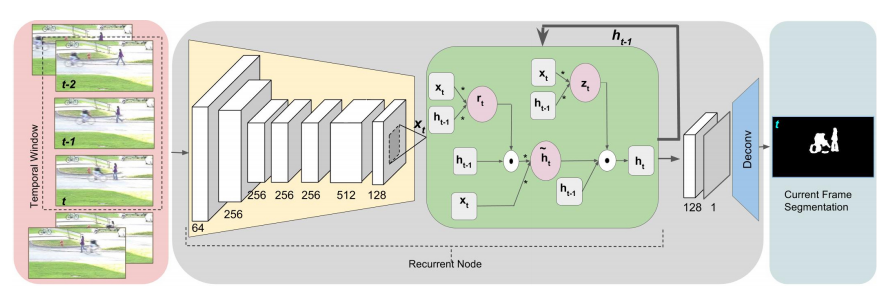
\includegraphics[scale=0.4]{recurrent_fcn.png} 
  \caption{The architecture of RFC-VGG from \cite{rFCN}. Images are fed frame by frame into a recurrent FCN. A Conv-GRU layer is applied on the feature maps produced by the preceding network at each frame.
The output of this layer goes to one more convolutional layer to generate heat maps. Finally, a
deconvolution layer up-samples the heat map to the desired spatial size.}
  \label{recurrent_fcn}
\end{figure}

\subsubsection{Recurrent Fully Convolutional Network}
Now to generate a video, we need to pass the contextual information from previous frames to the current frame so the frames are coherent to each other. For the discriminator network, we can do that using a regular LSTM network. The discriminator network generates a vector from the input images which can be transfered to the next instance of the discriminator. But the generator network is mostly a fully convolutional neural network, it is not straightforward to create a recursive model for the generator. We have considered the recurrent fully convolutional network \cite{rFCN} to solve this problem. The model uses convolutional gated recurrent units which establishes recurrent connections between the colvolutional layers. This model preserves the spatial information while passing context to the next LSTM unit and reduces the number oflearned parameters as well. The model is described in Figure \ref{recurrent_fcn}.

\begin{figure}[h]

  \centering
  %%\fbox{\rule[-.5cm]{0cm}{4cm} \rule[-.5cm]{4cm}{0cm}}
  \includegraphics[scale=0.5]{RSGAN.png} 
  \caption{The proposed Recurrent Stacked Generative network (RSGAN). The recurrent adversarial network modules at the first stage (RGAN-1) take the encoded pre-condition and a random vector $z_t$ and then produces a low resolution ($64 \times 64$) size image. The modules at stage-2 (RGAN-2) takes the generated image at stage-1 and the encoded pre-condition to generate a high resolution image ($256 \times 256$).}
    \label{RSGAN}
\end{figure}

\subsubsection{Recurrent Stacked Adversarial Network}
Now, we have the models to generate individual images from the pre-condition and also we can connect this individual adversarial networks using recurrent connection. We combine these two models and propose the Recurrent Stacked Generative network (RSGAN) for conditional video generation. The model expands both in the temporal and spatial dimension. Each module in the first stage takes the encoded pre-condition and a random vector as input and passes a contextual matrix to the next module to generate a low resolution frame sequence. Then the modules in the second stage takes the encoded pre-condition and the low resolution output from the previous stage to generate a high resolution video sequence. The model is described in Figure \ref{RSGAN}.


\subsubsection{Training} The model is trained using back propagation through time (bptt) and the usual adversarial training to train the recurrent generators and discriminators. 

\section{Experiments}
\label{experiments}
To evaluate our model we will conduct experiments on three video datasets.

\subsection{UCF-101 Dataset}
The UCF-101 \cite{uCF101} dataset contains short videos of 101 action classes. We will get the word-vector representation of the action class names and use those as the pre-conditions to generate the videos.

\subsection{VIM-2 Dataset}
VIM-2 dataset \cite{recVEBA} contains 7200 seconds of training and 540 seconds of test fMRI BOLD (blood oxygen level) signals and corresponding 15 frames of stimulation for each second. We will use the fMRI signals from the early visual area (V1, V2, V3, V3a, V3b) as our pre-condition to reproduce the video stimulations.

\subsection{Large Scale Movie Description Dataset}
Finally, we will use the Large Scale Movie Description Dataset \cite{movieDes} which contains 4-5 seconds videos from movies and their textual descriptions. We will use the Skip-Thought vector to encode the sentence descriptions and use them as pre-conditions.

\section{Evaluation}
As this is the first work on conditional video generation, we do not have a baseline or established evaluation criteria yet. We are still working on a reasonable evaluation criteria. Human evaluation can be an effective approach here.

\section{Conclusion}
We have proposed a novel adversarial network based model to generate videos based on a given condition. Our model can generate video frames which are coherent and consistent to the given condition. 

%\section*{References}
\small
\bibliographystyle{abbrv}
\bibliography{nips_2017}

\end{document}